% % Permutation 3
% middle3(X, [X]).
% middle3(X, [First|Xs]) :-
%   middle3(X, Middle),
%   append1(Middle, [Last], Xs).

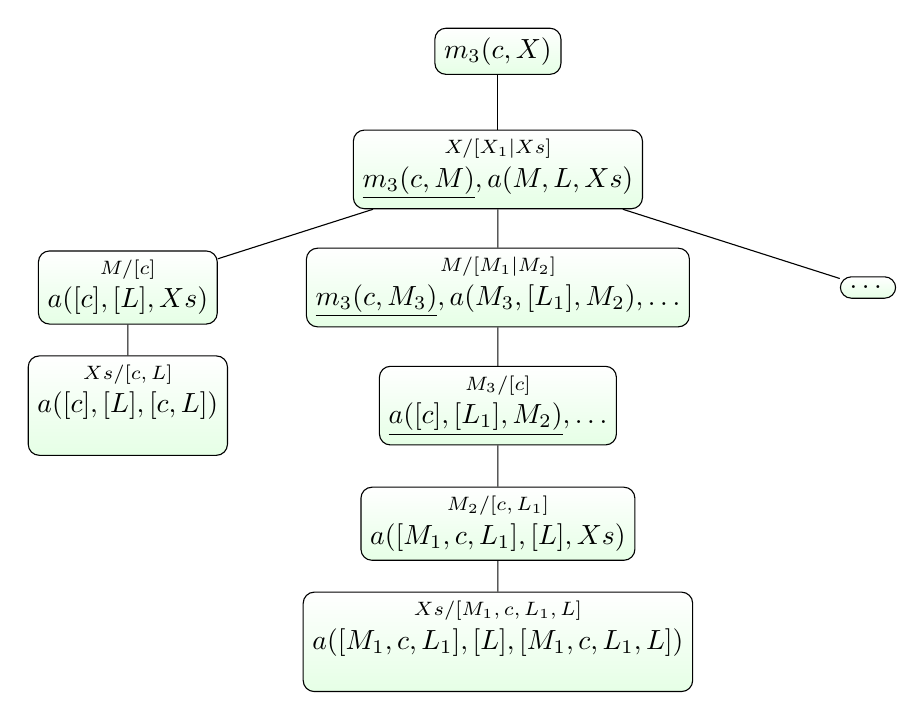
\begin{tikzpicture}[sibling distance=12em, align=center,
  every node/.style = {shape=rectangle, rounded corners,
    draw, align=center,
    top color=white, bottom color=green!10},
    level 1/.style={sibling distance=4cm},
    level 2/.style={sibling distance=4.7cm}, 
    level 3/.style={sibling distance=2.5cm}, ]
  \node {$m_3(c,X)$}
    child { node {\scriptsize $X/[X_1|Xs]$\\$\underline{m_3(c,M)},a(M,L,Xs)$}
      child {node {\scriptsize $M/[c]$\\$a([c],[L],Xs)$}
        child {node {\scriptsize $Xs/[c,L]$\\$a([c],[L],[c,L])$\\$\blacksquare$}}
      }
      child { node {\scriptsize $M/[M_1|M_2]$\\$\underline{m_3(c,M_3)},a(M_3,[L_1],M_2),\ldots$}
        child { node {\scriptsize $M_3/[c]$\\$\underline{a([c],[L_1],M_2)},\ldots$}
          child { node {\scriptsize $M_2/[c,L_1]$\\$a([M_1,c,L_1],[L],Xs)$}
            child {node {\scriptsize $Xs/[M_1,c,L_1,L]$\\$a([M_1,c,L_1],[L],[M_1,c,L_1,L])$\\$\blacksquare$}}
          }
        }
      }
      child { node {\ldots}}
    };
\end{tikzpicture}